\documentclass[twoside]{book}

% Packages required by doxygen
\usepackage{fixltx2e}
\usepackage{calc}
\usepackage{doxygen}
\usepackage[export]{adjustbox} % also loads graphicx
\usepackage{graphicx}
\usepackage[utf8]{inputenc}
\usepackage{makeidx}
\usepackage{multicol}
\usepackage{multirow}
\PassOptionsToPackage{warn}{textcomp}
\usepackage{textcomp}
\usepackage[nointegrals]{wasysym}
\usepackage[table]{xcolor}

% Font selection
\usepackage[T1]{fontenc}
\usepackage[scaled=.90]{helvet}
\usepackage{courier}
\usepackage{amssymb}
\usepackage{sectsty}
\renewcommand{\familydefault}{\sfdefault}
\allsectionsfont{%
  \fontseries{bc}\selectfont%
  \color{darkgray}%
}
\renewcommand{\DoxyLabelFont}{%
  \fontseries{bc}\selectfont%
  \color{darkgray}%
}
\newcommand{\+}{\discretionary{\mbox{\scriptsize$\hookleftarrow$}}{}{}}

% Page & text layout
\usepackage{geometry}
\geometry{%
  a4paper,%
  top=2.5cm,%
  bottom=2.5cm,%
  left=2.5cm,%
  right=2.5cm%
}
\tolerance=750
\hfuzz=15pt
\hbadness=750
\setlength{\emergencystretch}{15pt}
\setlength{\parindent}{0cm}
\setlength{\parskip}{3ex plus 2ex minus 2ex}
\makeatletter
\renewcommand{\paragraph}{%
  \@startsection{paragraph}{4}{0ex}{-1.0ex}{1.0ex}{%
    \normalfont\normalsize\bfseries\SS@parafont%
  }%
}
\renewcommand{\subparagraph}{%
  \@startsection{subparagraph}{5}{0ex}{-1.0ex}{1.0ex}{%
    \normalfont\normalsize\bfseries\SS@subparafont%
  }%
}
\makeatother

% Headers & footers
\usepackage{fancyhdr}
\pagestyle{fancyplain}
\fancyhead[LE]{\fancyplain{}{\bfseries\thepage}}
\fancyhead[CE]{\fancyplain{}{}}
\fancyhead[RE]{\fancyplain{}{\bfseries\leftmark}}
\fancyhead[LO]{\fancyplain{}{\bfseries\rightmark}}
\fancyhead[CO]{\fancyplain{}{}}
\fancyhead[RO]{\fancyplain{}{\bfseries\thepage}}
\fancyfoot[LE]{\fancyplain{}{}}
\fancyfoot[CE]{\fancyplain{}{}}
\fancyfoot[RE]{\fancyplain{}{\bfseries\scriptsize Generated by Doxygen }}
\fancyfoot[LO]{\fancyplain{}{\bfseries\scriptsize Generated by Doxygen }}
\fancyfoot[CO]{\fancyplain{}{}}
\fancyfoot[RO]{\fancyplain{}{}}
\renewcommand{\footrulewidth}{0.4pt}
\renewcommand{\chaptermark}[1]{%
  \markboth{#1}{}%
}
\renewcommand{\sectionmark}[1]{%
  \markright{\thesection\ #1}%
}

% Indices & bibliography
\usepackage{natbib}
\usepackage[titles]{tocloft}
\setcounter{tocdepth}{3}
\setcounter{secnumdepth}{5}
\makeindex

% Hyperlinks (required, but should be loaded last)
\usepackage{ifpdf}
\ifpdf
  \usepackage[pdftex,pagebackref=true]{hyperref}
\else
  \usepackage[ps2pdf,pagebackref=true]{hyperref}
\fi
\hypersetup{%
  colorlinks=true,%
  linkcolor=blue,%
  citecolor=blue,%
  unicode%
}

% Custom commands
\newcommand{\clearemptydoublepage}{%
  \newpage{\pagestyle{empty}\cleardoublepage}%
}

\usepackage{caption}
\captionsetup{labelsep=space,justification=centering,font={bf},singlelinecheck=off,skip=4pt,position=top}

%===== C O N T E N T S =====

\begin{document}

% Titlepage & ToC
\hypersetup{pageanchor=false,
             bookmarksnumbered=true,
             pdfencoding=unicode
            }
\pagenumbering{roman}
\begin{titlepage}
\vspace*{7cm}
\begin{center}%
{\Large Pepper\+\_\+tracking \\[1ex]\large 0.\+1 }\\
\vspace*{1cm}
{\large Generated by Doxygen 1.8.11}\\
\end{center}
\end{titlepage}
\clearemptydoublepage
\tableofcontents
\clearemptydoublepage
\pagenumbering{arabic}
\hypersetup{pageanchor=true}

%--- Begin generated contents ---
\chapter{Class Index}
\section{Class List}
Here are the classes, structs, unions and interfaces with brief descriptions\+:\begin{DoxyCompactList}
\item\contentsline{section}{\hyperlink{classauto_walking}{auto\+Walking} }{\pageref{classauto_walking}}{}
\item\contentsline{section}{\hyperlink{classsensor_info}{sensor\+Info} }{\pageref{classsensor_info}}{}
\end{DoxyCompactList}

\chapter{File Index}
\section{File List}
Here is a list of all files with brief descriptions\+:\begin{DoxyCompactList}
\item\contentsline{section}{/home/mis/follow\+\_\+ws/src/pepper\+\_\+tracking/src/\hyperlink{asker_8cpp}{asker.\+cpp} \\*Do the bridge between the user ask and the image worker }{\pageref{asker_8cpp}}{}
\item\contentsline{section}{/home/mis/follow\+\_\+ws/src/pepper\+\_\+tracking/src/\hyperlink{worker_8cpp}{worker.\+cpp} \\*Do the bridge between visp, pepper and the user node }{\pageref{worker_8cpp}}{}
\end{DoxyCompactList}

\chapter{Class Documentation}
\hypertarget{classasker}{}\section{asker Class Reference}
\label{classasker}\index{asker@{asker}}


Allow the user to add/remove image to the list of goals of Pepper.  


\subsection*{Public Member Functions}
\begin{DoxyCompactItemize}
\item 
\hyperlink{classasker_a38f92b2656bc29658461ba95c846e63a}{asker} ()
\item 
void \hyperlink{classasker_a8f975187b555b7f6d47fbf4d31788d9b}{image\+Return} (const pepper\+\_\+tracking\+::image\+\_\+return \&msg)
\begin{DoxyCompactList}\small\item\em Receive the callback of the worker concerning a goal success. \end{DoxyCompactList}\item 
void \hyperlink{classasker_a4c549520b5964424716f28f1753517ad}{add\+Image} (sensor\+\_\+msgs\+::\+Image new\+Image, std\+::string image\+Name)
\begin{DoxyCompactList}\small\item\em Sending image searching request to the topic. \end{DoxyCompactList}\item 
void \hyperlink{classasker_acb07a6a00d25ae3df55ae18583ebfdb3}{remove\+Image} (std\+::string image\+Name)
\begin{DoxyCompactList}\small\item\em When an image found is receive, publish the success. \end{DoxyCompactList}\end{DoxyCompactItemize}


\subsection{Detailed Description}
Allow the user to add/remove image to the list of goals of Pepper. 

Definition at line 27 of file asker.\+cpp.



\subsection{Constructor \& Destructor Documentation}
\index{asker@{asker}!asker@{asker}}
\index{asker@{asker}!asker@{asker}}
\subsubsection[{\texorpdfstring{asker()}{asker()}}]{\setlength{\rightskip}{0pt plus 5cm}asker\+::asker (
\begin{DoxyParamCaption}
{}
\end{DoxyParamCaption}
)\hspace{0.3cm}{\ttfamily [inline]}}\hypertarget{classasker_a38f92b2656bc29658461ba95c846e63a}{}\label{classasker_a38f92b2656bc29658461ba95c846e63a}


Definition at line 33 of file asker.\+cpp.



\subsection{Member Function Documentation}
\index{asker@{asker}!add\+Image@{add\+Image}}
\index{add\+Image@{add\+Image}!asker@{asker}}
\subsubsection[{\texorpdfstring{add\+Image(sensor\+\_\+msgs\+::\+Image new\+Image, std\+::string image\+Name)}{addImage(sensor_msgs::Image newImage, std::string imageName)}}]{\setlength{\rightskip}{0pt plus 5cm}void asker\+::add\+Image (
\begin{DoxyParamCaption}
\item[{sensor\+\_\+msgs\+::\+Image}]{new\+Image, }
\item[{std\+::string}]{image\+Name}
\end{DoxyParamCaption}
)\hspace{0.3cm}{\ttfamily [inline]}}\hypertarget{classasker_a4c549520b5964424716f28f1753517ad}{}\label{classasker_a4c549520b5964424716f28f1753517ad}


Sending image searching request to the topic. 

Other function


\begin{DoxyParams}{Parameters}
{\em new\+Image} & The image on a sensor\+\_\+msgs\+::\+Image format \\
\hline
{\em image\+Name} & Used as id for the new image \\
\hline
\end{DoxyParams}
\begin{DoxyReturn}{Returns}
void 
\end{DoxyReturn}


Definition at line 73 of file asker.\+cpp.

\index{asker@{asker}!image\+Return@{image\+Return}}
\index{image\+Return@{image\+Return}!asker@{asker}}
\subsubsection[{\texorpdfstring{image\+Return(const pepper\+\_\+tracking\+::image\+\_\+return \&msg)}{imageReturn(const pepper_tracking::image_return &msg)}}]{\setlength{\rightskip}{0pt plus 5cm}void asker\+::image\+Return (
\begin{DoxyParamCaption}
\item[{const pepper\+\_\+tracking\+::image\+\_\+return \&}]{msg}
\end{DoxyParamCaption}
)\hspace{0.3cm}{\ttfamily [inline]}}\hypertarget{classasker_a8f975187b555b7f6d47fbf4d31788d9b}{}\label{classasker_a8f975187b555b7f6d47fbf4d31788d9b}


Receive the callback of the worker concerning a goal success. 

Subcriber Call\+Back


\begin{DoxyParams}{Parameters}
{\em msg} & Custom msg from this package, pepper\+\_\+tracking/image\+\_\+return.\+msg \\
\hline
\end{DoxyParams}
\begin{DoxyReturn}{Returns}
void 
\end{DoxyReturn}


Definition at line 58 of file asker.\+cpp.

\index{asker@{asker}!remove\+Image@{remove\+Image}}
\index{remove\+Image@{remove\+Image}!asker@{asker}}
\subsubsection[{\texorpdfstring{remove\+Image(std\+::string image\+Name)}{removeImage(std::string imageName)}}]{\setlength{\rightskip}{0pt plus 5cm}void asker\+::remove\+Image (
\begin{DoxyParamCaption}
\item[{std\+::string}]{image\+Name}
\end{DoxyParamCaption}
)\hspace{0.3cm}{\ttfamily [inline]}}\hypertarget{classasker_acb07a6a00d25ae3df55ae18583ebfdb3}{}\label{classasker_acb07a6a00d25ae3df55ae18583ebfdb3}


When an image found is receive, publish the success. 


\begin{DoxyParams}{Parameters}
{\em image\+Name} & Used as id for the image \\
\hline
\end{DoxyParams}
\begin{DoxyReturn}{Returns}
void 
\end{DoxyReturn}


Definition at line 91 of file asker.\+cpp.



The documentation for this class was generated from the following file\+:\begin{DoxyCompactItemize}
\item 
/home/mis/follow\+\_\+ws/src/pepper\+\_\+tracking/src/\hyperlink{asker_8cpp}{asker.\+cpp}\end{DoxyCompactItemize}

\hypertarget{classworker}{}\section{worker Class Reference}
\label{classworker}\index{worker@{worker}}


Allow Pepper to move and detect user wanted image.  


\subsection*{Public Member Functions}
\begin{DoxyCompactItemize}
\item 
\hyperlink{classworker_a7bd845810dd8185384e37405ef322b7d}{worker} ()
\item 
void \hyperlink{classworker_a8f0d3d3cbd7418830cd77a0bba55465b}{image\+Request} (const pepper\+\_\+tracking\+::image\+\_\+request \&msg)
\begin{DoxyCompactList}\small\item\em Receive the new image request to find in the area. \end{DoxyCompactList}\item 
void \hyperlink{classworker_a24193ed917b818ef20de0240499468fc}{image\+Raw} (const sensor\+\_\+msgs\+::\+Image \&msg)
\begin{DoxyCompactList}\small\item\em Allow to process the image\+\_\+raw of Pepper. \end{DoxyCompactList}\item 
void \hyperlink{classworker_a2accc661aa0de65223603bfff5f69b27}{request\+To\+Visp} (sensor\+\_\+msgs\+::\+Image image\+Goal, sensor\+\_\+msgs\+::\+Image image\+Nao)
\begin{DoxyCompactList}\small\item\em In charge of doing the request to compare both image to V\+Isp. \end{DoxyCompactList}\item 
void \hyperlink{classworker_a27863e3e984867effbc8accfb0d034f8}{image\+Found} (std\+::string image\+Name)
\begin{DoxyCompactList}\small\item\em When Visp say that two image are similar, publish the success. \end{DoxyCompactList}\end{DoxyCompactItemize}


\subsection{Detailed Description}
Allow Pepper to move and detect user wanted image. 

Definition at line 26 of file worker.\+cpp.



\subsection{Constructor \& Destructor Documentation}
\index{worker@{worker}!worker@{worker}}
\index{worker@{worker}!worker@{worker}}
\subsubsection[{\texorpdfstring{worker()}{worker()}}]{\setlength{\rightskip}{0pt plus 5cm}worker\+::worker (
\begin{DoxyParamCaption}
{}
\end{DoxyParamCaption}
)\hspace{0.3cm}{\ttfamily [inline]}}\hypertarget{classworker_a7bd845810dd8185384e37405ef322b7d}{}\label{classworker_a7bd845810dd8185384e37405ef322b7d}


Definition at line 29 of file worker.\+cpp.



\subsection{Member Function Documentation}
\index{worker@{worker}!image\+Found@{image\+Found}}
\index{image\+Found@{image\+Found}!worker@{worker}}
\subsubsection[{\texorpdfstring{image\+Found(std\+::string image\+Name)}{imageFound(std::string imageName)}}]{\setlength{\rightskip}{0pt plus 5cm}void worker\+::image\+Found (
\begin{DoxyParamCaption}
\item[{std\+::string}]{image\+Name}
\end{DoxyParamCaption}
)\hspace{0.3cm}{\ttfamily [inline]}}\hypertarget{classworker_a27863e3e984867effbc8accfb0d034f8}{}\label{classworker_a27863e3e984867effbc8accfb0d034f8}


When Visp say that two image are similar, publish the success. 


\begin{DoxyParams}{Parameters}
{\em image\+Name} & Id/\+Name of the image found to inform the topic \\
\hline
\end{DoxyParams}
\begin{DoxyReturn}{Returns}
void 
\end{DoxyReturn}


Definition at line 104 of file worker.\+cpp.

\index{worker@{worker}!image\+Raw@{image\+Raw}}
\index{image\+Raw@{image\+Raw}!worker@{worker}}
\subsubsection[{\texorpdfstring{image\+Raw(const sensor\+\_\+msgs\+::\+Image \&msg)}{imageRaw(const sensor_msgs::Image &msg)}}]{\setlength{\rightskip}{0pt plus 5cm}void worker\+::image\+Raw (
\begin{DoxyParamCaption}
\item[{const sensor\+\_\+msgs\+::\+Image \&}]{msg}
\end{DoxyParamCaption}
)\hspace{0.3cm}{\ttfamily [inline]}}\hypertarget{classworker_a24193ed917b818ef20de0240499468fc}{}\label{classworker_a24193ed917b818ef20de0240499468fc}


Allow to process the image\+\_\+raw of Pepper. 


\begin{DoxyParams}{Parameters}
{\em msg} & Pepper camera output \\
\hline
\end{DoxyParams}
\begin{DoxyReturn}{Returns}
void 
\end{DoxyReturn}


Definition at line 78 of file worker.\+cpp.

\index{worker@{worker}!image\+Request@{image\+Request}}
\index{image\+Request@{image\+Request}!worker@{worker}}
\subsubsection[{\texorpdfstring{image\+Request(const pepper\+\_\+tracking\+::image\+\_\+request \&msg)}{imageRequest(const pepper_tracking::image_request &msg)}}]{\setlength{\rightskip}{0pt plus 5cm}void worker\+::image\+Request (
\begin{DoxyParamCaption}
\item[{const pepper\+\_\+tracking\+::image\+\_\+request \&}]{msg}
\end{DoxyParamCaption}
)\hspace{0.3cm}{\ttfamily [inline]}}\hypertarget{classworker_a8f0d3d3cbd7418830cd77a0bba55465b}{}\label{classworker_a8f0d3d3cbd7418830cd77a0bba55465b}


Receive the new image request to find in the area. 

Subcriber Call\+Back


\begin{DoxyParams}{Parameters}
{\em msg} & Custom msg from this package, pepper\+\_\+tracking/image\+\_\+request.\+msg \\
\hline
\end{DoxyParams}
\begin{DoxyReturn}{Returns}
void 
\end{DoxyReturn}


Definition at line 51 of file worker.\+cpp.

\index{worker@{worker}!request\+To\+Visp@{request\+To\+Visp}}
\index{request\+To\+Visp@{request\+To\+Visp}!worker@{worker}}
\subsubsection[{\texorpdfstring{request\+To\+Visp(sensor\+\_\+msgs\+::\+Image image\+Goal, sensor\+\_\+msgs\+::\+Image image\+Nao)}{requestToVisp(sensor_msgs::Image imageGoal, sensor_msgs::Image imageNao)}}]{\setlength{\rightskip}{0pt plus 5cm}void worker\+::request\+To\+Visp (
\begin{DoxyParamCaption}
\item[{sensor\+\_\+msgs\+::\+Image}]{image\+Goal, }
\item[{sensor\+\_\+msgs\+::\+Image}]{image\+Nao}
\end{DoxyParamCaption}
)\hspace{0.3cm}{\ttfamily [inline]}}\hypertarget{classworker_a2accc661aa0de65223603bfff5f69b27}{}\label{classworker_a2accc661aa0de65223603bfff5f69b27}


In charge of doing the request to compare both image to V\+Isp. 


\begin{DoxyParams}{Parameters}
{\em image\+Goal} & All image that we want to find, one by one \\
\hline
{\em image\+Nao} & A frame of pepper vision \\
\hline
\end{DoxyParams}
\begin{DoxyReturn}{Returns}
void 
\end{DoxyReturn}


Definition at line 93 of file worker.\+cpp.



The documentation for this class was generated from the following file\+:\begin{DoxyCompactItemize}
\item 
/home/mis/follow\+\_\+ws/src/pepper\+\_\+tracking/src/\hyperlink{worker_8cpp}{worker.\+cpp}\end{DoxyCompactItemize}

\chapter{File Documentation}
\hypertarget{asker_8cpp}{}\section{/home/mis/follow\+\_\+ws/src/pepper\+\_\+tracking/src/asker.cpp File Reference}
\label{asker_8cpp}\index{/home/mis/follow\+\_\+ws/src/pepper\+\_\+tracking/src/asker.\+cpp@{/home/mis/follow\+\_\+ws/src/pepper\+\_\+tracking/src/asker.\+cpp}}


Do the bridge between the user ask and the image worker.  


{\ttfamily \#include $<$ros/ros.\+h$>$}\\*
{\ttfamily \#include $<$sensor\+\_\+msgs/\+Image.\+h$>$}\\*
{\ttfamily \#include $<$pepper\+\_\+tracking/image\+\_\+request.\+h$>$}\\*
{\ttfamily \#include $<$pepper\+\_\+tracking/image\+\_\+return.\+h$>$}\\*
{\ttfamily \#include $<$time.\+h$>$}\\*
{\ttfamily \#include $<$string.\+h$>$}\\*
{\ttfamily \#include $<$vector$>$}\\*
Include dependency graph for asker.\+cpp\+:\nopagebreak
\begin{figure}[H]
\begin{center}
\leavevmode
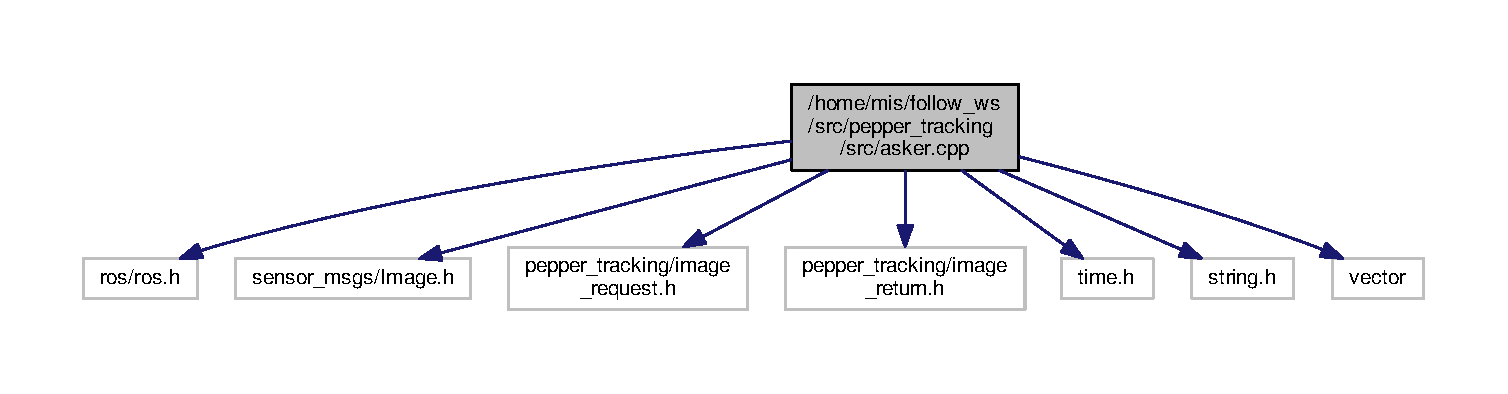
\includegraphics[width=350pt]{asker_8cpp__incl}
\end{center}
\end{figure}
\subsection*{Classes}
\begin{DoxyCompactItemize}
\item 
class \hyperlink{classasker}{asker}
\begin{DoxyCompactList}\small\item\em Allow the user to add/remove image to the list of goals of Pepper. \end{DoxyCompactList}\end{DoxyCompactItemize}
\subsection*{Functions}
\begin{DoxyCompactItemize}
\item 
int \hyperlink{asker_8cpp_a3c04138a5bfe5d72780bb7e82a18e627}{main} (int argc, char $\ast$$\ast$argv)
\end{DoxyCompactItemize}


\subsection{Detailed Description}
Do the bridge between the user ask and the image worker. 

\begin{DoxyAuthor}{Author}
Vivien.\+C 
\end{DoxyAuthor}
\begin{DoxyDate}{Date}
02/05/2018
\end{DoxyDate}
The user input an image in a special format, and this node ask to find the area of this image if it\textquotesingle{}s possible. 

\subsection{Function Documentation}
\index{asker.\+cpp@{asker.\+cpp}!main@{main}}
\index{main@{main}!asker.\+cpp@{asker.\+cpp}}
\subsubsection[{\texorpdfstring{main(int argc, char $\ast$$\ast$argv)}{main(int argc, char **argv)}}]{\setlength{\rightskip}{0pt plus 5cm}int main (
\begin{DoxyParamCaption}
\item[{int}]{argc, }
\item[{char $\ast$$\ast$}]{argv}
\end{DoxyParamCaption}
)}\hypertarget{asker_8cpp_a3c04138a5bfe5d72780bb7e82a18e627}{}\label{asker_8cpp_a3c04138a5bfe5d72780bb7e82a18e627}


Definition at line 117 of file asker.\+cpp.


\hypertarget{worker_8cpp}{}\section{/home/mis/follow\+\_\+ws/src/pepper\+\_\+tracking/src/worker.cpp File Reference}
\label{worker_8cpp}\index{/home/mis/follow\+\_\+ws/src/pepper\+\_\+tracking/src/worker.\+cpp@{/home/mis/follow\+\_\+ws/src/pepper\+\_\+tracking/src/worker.\+cpp}}


Do the bridge between visp, pepper and the user node.  


{\ttfamily \#include $<$ros/ros.\+h$>$}\\*
{\ttfamily \#include $<$sensor\+\_\+msgs/\+Image.\+h$>$}\\*
{\ttfamily \#include $<$pepper\+\_\+tracking/image\+\_\+request.\+h$>$}\\*
{\ttfamily \#include $<$pepper\+\_\+tracking/image\+\_\+return.\+h$>$}\\*
{\ttfamily \#include $<$time.\+h$>$}\\*
{\ttfamily \#include $<$string.\+h$>$}\\*
{\ttfamily \#include $<$vector$>$}\\*
Include dependency graph for worker.\+cpp\+:\nopagebreak
\begin{figure}[H]
\begin{center}
\leavevmode
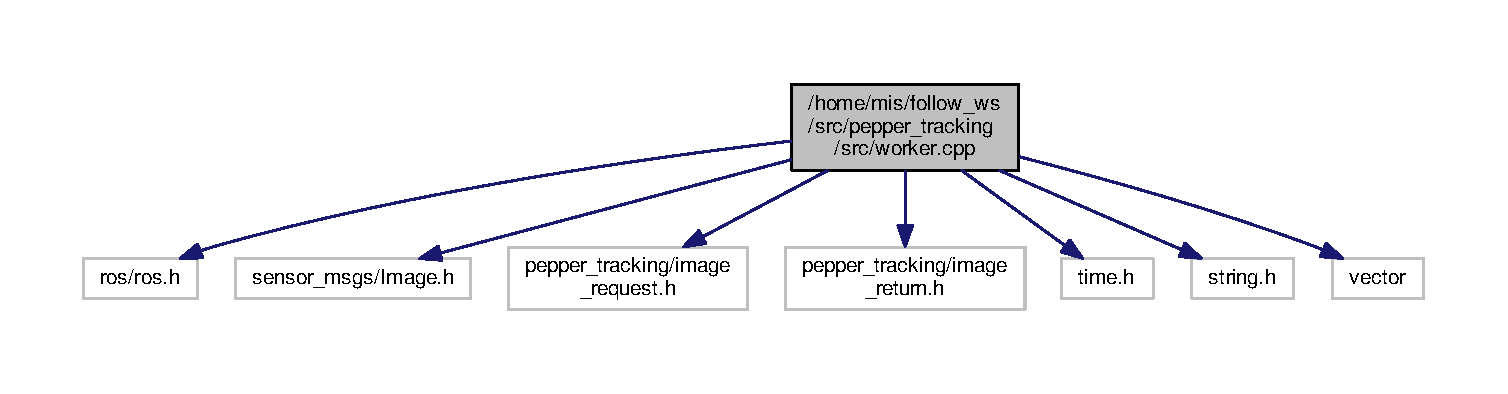
\includegraphics[width=350pt]{worker_8cpp__incl}
\end{center}
\end{figure}
\subsection*{Classes}
\begin{DoxyCompactItemize}
\item 
class \hyperlink{classworker}{worker}
\begin{DoxyCompactList}\small\item\em Allow Pepper to move and detect user wanted image. \end{DoxyCompactList}\end{DoxyCompactItemize}
\subsection*{Functions}
\begin{DoxyCompactItemize}
\item 
int \hyperlink{worker_8cpp_a3c04138a5bfe5d72780bb7e82a18e627}{main} (int argc, char $\ast$$\ast$argv)
\end{DoxyCompactItemize}


\subsection{Detailed Description}
Do the bridge between visp, pepper and the user node. 

\begin{DoxyAuthor}{Author}
Vivien.\+C 
\end{DoxyAuthor}
\begin{DoxyDate}{Date}
02/05/2018
\end{DoxyDate}
Allow Pepper to find in the area an image ask by user 

\subsection{Function Documentation}
\index{worker.\+cpp@{worker.\+cpp}!main@{main}}
\index{main@{main}!worker.\+cpp@{worker.\+cpp}}
\subsubsection[{\texorpdfstring{main(int argc, char $\ast$$\ast$argv)}{main(int argc, char **argv)}}]{\setlength{\rightskip}{0pt plus 5cm}int main (
\begin{DoxyParamCaption}
\item[{int}]{argc, }
\item[{char $\ast$$\ast$}]{argv}
\end{DoxyParamCaption}
)}\hypertarget{worker_8cpp_a3c04138a5bfe5d72780bb7e82a18e627}{}\label{worker_8cpp_a3c04138a5bfe5d72780bb7e82a18e627}


Definition at line 131 of file worker.\+cpp.


%--- End generated contents ---

% Index
\backmatter
\newpage
\phantomsection
\clearemptydoublepage
\addcontentsline{toc}{chapter}{Index}
\printindex

\end{document}
